\documentclass[12pt, letterpaper]{article}
\usepackage[utf8]{inputenc}
\usepackage[margin=2cm]{geometry}
\usepackage{amsmath}
\usepackage{amssymb}
\usepackage{graphicx}
\usepackage{cancel}
\usepackage{fancyhdr}
\usepackage{float}

\graphicspath{ {./bilder/} }

\title{ \begin{huge}
\textbf{Portfolio Assignment 3}
\end{huge} }

\author{Candidate 25}
\date{}

\rfoot{\thepage}
\newcommand{\bs}{\boldsymbol}
\newcommand{\mbf}{\mathbf}

\begin{document}
\maketitle
  \section*{Problem 1}
    \subsection*{(1a)}
        I shall now discuss the main difference between feature extraction and feature selection. HEllo 

    %   \begin{figure}[H]
    %     \caption{Decision boudary of a logistic descrimination classifier}
    %     \centering
    %     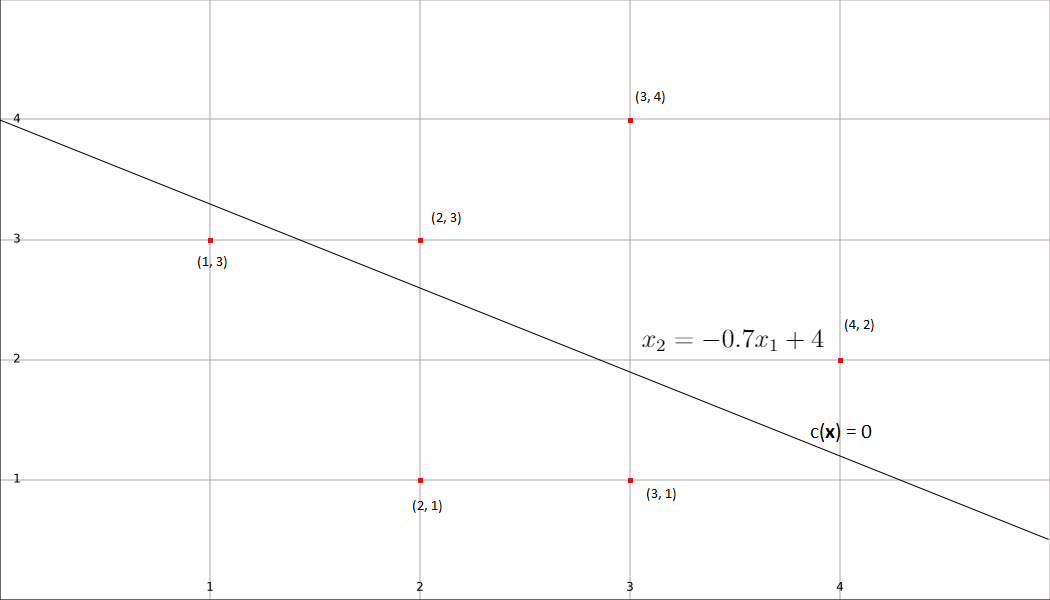
\includegraphics[width=\textwidth,keepaspectratio=true,height=\textheight-\the\textundbildtextheight]{decisionboundary_1a}
    %   \end{figure}\\
\end{document}
